%% Supplementary Information for the Matters Arising
%% "Two identifiability gaps in inferring symmetric critical dynamics
%%  from cortical population activity"
%% Standalone; compile:  pdflatex matters_arising_v4_supp -> bibtex -> pdflatex x2
\documentclass[11pt]{article}
\usepackage[margin=1in]{geometry}
\usepackage{amsmath,amssymb}
\usepackage{graphicx}
\usepackage{booktabs}
\usepackage{multirow}
\usepackage[hidelinks]{hyperref}

\newcommand{\alphaeff}{\alpha_{\mathrm{eff}}}
\newcommand{\asym}{\mathcal{A}}
\renewcommand{\thesection}{S\arabic{section}}
\renewcommand{\thetable}{S\arabic{table}}
\renewcommand{\thefigure}{S\arabic{figure}}
\renewcommand{\theequation}{S\arabic{equation}}

\title{Supplementary Information\\[4pt]
\large Cortical population activity does not identify symmetric critical
dynamics}
\author{}
\date{}

\begin{document}
\maketitle
\vspace{-3em}

\tableofcontents
\bigskip

%====================================================================
\section{The two identifiability gaps: summary}
\label{sec:summary}

The original Article\cite{pachitariu2026} reports two main observables from
spontaneous cortical activity: a covariance power-law exponent
$\nu\approx 0.7$--$0.85$, and near-real DMD eigenvalues. These observables are
interpreted as evidence that the underlying effective dynamics are symmetric and
critically normalized. This Supplementary Information provides the full derivations and
data for two linked identifiability gaps:

\begin{enumerate}
  \item \textbf{The exponent is degenerate} (Sec.~\ref{sec:degeneracy}):
    within a controlled elliptic-law family, $\nu$ varies jointly with at least
    two latent operator properties---reciprocity $\eta$ and continuous-time spectral abscissa
    $\alphaeff=\max\operatorname{Re}\lambda(A)$---and the same $\nu$ is
    produced by a continuum of $(\eta,\alphaeff)$ pairs. This constructive
    two-parameter degeneracy is sufficient: the exponent alone
    therefore does not establish distance to the stability boundary.
  \item \textbf{The DMD spectrum does not identify symmetry}
    (Sec.~\ref{sec:counterexample}): a non-symmetric, non-normal operator can
    have an entirely real spectrum through similarity transformation. A
    constructive counterexample reproduces the eigenvalue-level signature used
    to infer symmetry while retaining the relevant covariance and memory
    benchmarks.
\end{enumerate}

Together, these gaps imply that neither measurement separately identifies its
target property, and they do not mutually resolve. The supported conclusion is
low-modal-rotation effective dynamics whose covariance spectrum is compatible
with a family of reciprocity--criticality combinations, not a unique symmetric
critical operator (Sec.~\ref{sec:synthesis}). Both gaps are then confirmed
empirically in a whole-brain spiking model with structural ground truth
(Sec.~\ref{sec:flywire}): when reciprocity is varied over two orders of magnitude
at fixed degree, neither the DMD spectrum nor the covariance exponent recovers
it.

%====================================================================
\section{Linear dynamics and the stationary covariance}
\label{sec:linear}

We use the continuous-time linear model of the original Article,
\begin{equation}
\tau\frac{dx}{dt}=(-I+A)x+\xi(t),\qquad
\langle\xi_i(t)\xi_j(t')\rangle = \sigma^2\delta_{ij}\delta(t-t').
\end{equation}
After absorbing $\tau$ into the noise scale, the stationary covariance solves
\begin{equation}
(A-I)\Sigma+\Sigma(A-I)^\top=-\sigma^2 I. \label{eq:lyap_ct}
\end{equation}
Stability requires $\alphaeff=\max\operatorname{Re}\lambda(A)<1$. The
principal-component variance spectrum is the sorted eigenvalue sequence of
$\Sigma$; its power-law index $\nu$ ($C_n\propto n^{-\nu}$) is the statistic at
issue. For symmetric $A$, Eq.~\eqref{eq:lyap_ct} diagonalises in the eigenbasis
of $A$, giving $C(\mu)=\sigma^2/[2(1-\mu)]$. For non-normal $A$ we solve the
continuous Lyapunov equation directly. The isotropic-white-drive assumption is
deliberately restrictive; structured or colored drive introduces additional
non-identifiability.

%====================================================================
\section{Gap~1: The exponent degeneracy \texorpdfstring{$\nu(\eta,\alphaeff)$}{nu(eta, alpha_eff)}}
\label{sec:degeneracy}

\subsection{The symmetric critical limit: derivation of \texorpdfstring{$\nu=2/3$}{ν=2/3}}
For symmetric $A$, Eq.~\eqref{eq:lyap_ct} diagonalises in the eigenbasis of
$A$ and the PC variance spectrum is the push-forward of the eigenvalue density
through $C(\mu)=\sigma^2/[2(1-\mu)]$. Let the eigenvalues follow the Wigner
semicircle on $[-\alphaeff,\alphaeff]$,
\begin{equation}
p(\mu)=\frac{2}{\pi\alphaeff^2}\sqrt{\alphaeff^2-\mu^2},
\qquad |\mu|\le\alphaeff .
\end{equation}
Ordering eigenvalues from the top edge downward, the rank $n$ of eigenvalue
$\mu$ is the upper-tail mass $n/N=\int_\mu^{\alphaeff}p(\mu')\,d\mu'$. Writing
$\mu=\alphaeff-\epsilon$ and using the square-root edge,
\begin{equation}
\frac{n}{N}\propto\int_0^{\epsilon}\!\sqrt{\epsilon'}\,d\epsilon'
\propto\epsilon^{3/2}
\propto(\alphaeff-\mu)^{3/2},
\label{eq:rankedge}
\end{equation}
so the singly-integrated square-root edge gives
$\alphaeff-\mu\propto(n/N)^{2/3}$. At the stability boundary the variance map
develops a pole: using $\alphaeff\to1$ and
$\mu\to1$,
\begin{equation}
C(\mu)=\frac{\sigma^2}{2(1-\mu)}
\simeq\frac{\sigma^2}{2(\alphaeff-\mu)},
\end{equation}
and combining with Eq.~\eqref{eq:rankedge},
\begin{equation}
\boxed{\,C_n\;\propto\;\frac{1}{\alphaeff-\mu}\;\propto\;
\left(\frac{n}{N}\right)^{-2/3}\qquad(\alphaeff\to1).\,}
\end{equation}
The exponent $\nu=2/3$ thus requires \emph{two} ingredients simultaneously: the
square-root vanishing of a \emph{symmetric} (Wigner) spectral edge
[Eq.~\eqref{eq:rankedge}], and the pole of $C(\mu)$ as $\mu\to1$
(\emph{criticality}). Relaxing either moves the exponent --- the origin of the
degeneracy below. Away from the boundary the pole saturates at
$\sigma^2/[2(1-\alphaeff)]$ over a low-rank plateau of width
$n_c\sim N(1-\alphaeff)^{3/2}$. A finite fitted rank window samples a mixture
of this plateau and the edge tail, so its fitted exponent depends on both
$\eta$ and $\alphaeff$.

\subsection{Reciprocity (elliptic-law) parameter}
We control the symmetry of $A$ with the Sommers--Crisanti--Sompolinsky--Stein
reciprocity parameter\cite{sommers1988}
$\eta=\langle A_{ij}A_{ji}\rangle/\langle A_{ij}^2\rangle\in[-1,1]$,
realised by drawing each off-diagonal pair as a correlated Gaussian:
\begin{equation}
A_{ij}=a_{ij},\qquad A_{ji}=\eta\,a_{ij}+\sqrt{1-\eta^2}\,b_{ij},
\qquad a,b\ \text{i.i.d.}\ \mathcal N(0,1/N),
\end{equation}
so that $\eta=1$ is symmetric (real spectrum), $\eta=0$ is independent
(Ginibre/circular law), and $\eta=-1$ is antisymmetric. Each operator is then
rescaled so that its spectral abscissa is $\alphaeff<1$.

\subsection{Why the exponent depends on reciprocity: the elliptic law}
Reciprocity enters the exponent because it controls the \emph{shape} of the
spectral edge. For the Gaussian elliptic ensemble the eigenvalues fill, as
$N\to\infty$, an ellipse in the complex plane with semi-axes
\begin{equation}
a=(1+\eta)\,s,\qquad b=(1-\eta)\,s
\end{equation}
along the real and imaginary directions, with $s$ fixing the overall
scale\cite{sommers1988}; after rescaling, the rightmost real part is
$\alphaeff$. Two limits bracket the family analytically. At $\eta=1$ the
ellipse collapses onto the real segment $[-\alphaeff,\alphaeff]$ with
the Wigner square-root edge, and the diagonal Lyapunov solution
$C(\mu)=\sigma^2/[2(1-\mu)]$ of the previous subsection applies, giving
$\nu\to2/3$. At $\eta=0$ the spectrum is the full Ginibre disk; the operator is
fully asymmetric and non-normal, the covariance no longer diagonalises in the
eigenbasis,
and solving Eq.~\eqref{eq:lyap_ct} directly gives a steeper fitted exponent
near the boundary. For intermediate $0<\eta<1$ the spectrum is a genuine
ellipse with a $b/a=(1-\eta)/(1+\eta)$ imaginary spread, the operator is
non-normal, and the exponent obtained from the direct Lyapunov solution
varies between the two endpoints. The single scalar $\nu$
therefore encodes a \emph{combination} of edge shape (reciprocity $\eta$) and
edge location (spectral abscissa $\alphaeff$) and cannot separate them.

\subsection{Degeneracy surface}
We solve Eq.~\eqref{eq:lyap_ct} on a grid of $(\eta,\alphaeff)$ and fit the
covariance spectrum with the Article's $1/\mathrm{rank}$-weighted log--log
regression over ranks 10--500, or half the available spectrum
(\texttt{ma\_degeneracy\_surface.py}). The symmetric column approaches
$\nu=2/3$ as $\alphaeff\to1$, whereas lower-reciprocity columns can produce
steeper exponents at the same abscissa. Iso-$\nu$ contours therefore run across
the $(\eta,\alphaeff)$ plane: the cortical exponent band constrains a family of
reciprocity--criticality combinations rather than identifying a unique point.
Finite-size and fitted-window effects shift individual values, so the code
reports the full grid, seeds, rank window and uncertainty rather than treating
an endpoint exponent as an exact structural estimator.

%====================================================================
\section{Gap~2: Real-spectrum non-normal counterexample}
\label{sec:counterexample}

\subsection{The identifiability issue}
The original Article compares two random-matrix ensembles: a symmetric ensemble
with real eigenvalues and an independent non-symmetric ensemble with a circular
complex spectrum. DMD separates those two ensembles because their rotational
content differs. This comparison does not establish the converse implication
\[
  \text{near-real DMD eigenvalues}\quad\Longrightarrow\quad
  \text{near-symmetric interactions}.
\]
Real symmetric matrices are one subclass of real-spectrum matrices. A
non-symmetric matrix can have a completely real spectrum, and a non-normal
matrix can be diagonalizable with a real spectrum. Our construction isolates
this logical gap while retaining the near-boundary eigenvalue distribution of
the original model.

\subsection{Real-spectrum non-normal construction}
For every realization, we draw a centred symmetric random matrix $S=S^\top$
and scale it so that $\lambda_{\max}(S)=0.998$. Let
\begin{equation}
  T_g=Q\,\mathrm{diag}(e^{g z_1},\ldots,e^{g z_N})Q^\top,
  \qquad A_g=T_g S T_g^{-1},
  \label{eq:construction}
\end{equation}
where $Q$ is Haar-random orthogonal, $z_i$ are standardized independent
Gaussian variables and $g\geq0$. The matrix $T_g$ is positive definite but
non-orthogonal for $g>0$. Consequently $A_g$ is similar to $S$ and has exactly
the same eigenvalues, but is generically non-symmetric and non-normal.

We report the Frobenius asymmetry
\begin{equation}
  \asym(A)=\frac{\lVert A-A^\top\rVert_F}{2\lVert A\rVert_F}
\end{equation}
and reciprocity
\begin{equation}
  \eta(A)=
  \frac{2\sum_{i<j}A_{ij}A_{ji}}
       {\sum_{i<j}(A_{ij}^2+A_{ji}^2)}.
\end{equation}
Symmetric matrices have $\asym=0$ and $\eta=1$. The main $g=0.30$
counterexample has $\asym=0.388$ and $\eta=0.698$ with a moderate transform
condition number of $6.04\pm1.38$ (Table~\ref{tab:operator}).

\subsection{DMD rotation is invariant under the counterexample}
For a DMD eigenvalue $\mu=|\mu|e^{i\varphi}$ (with $|\mu|<1$), the Article's
``rotations per tenfold attenuation'' is the number of full phase turns the mode
$e^{i\varphi t}$ completes while its amplitude $|\mu|^t$ decays by a factor of
ten:
\begin{equation}
\mathrm{rot}(\mu)=\frac{|\varphi|}{2\pi}\cdot\frac{\ln 10}{\ln(1/|\mu|)} .
\label{eq:rot}
\end{equation}
A real, positive eigenvalue has $\varphi=0$ and hence $\mathrm{rot}=0$; the
statistic is therefore set entirely by the phases of the DMD spectrum.

At delay $\Delta t$, the noise-free DMD operator is
\begin{align}
  B_g
  &=\exp[(A_g-I)\Delta t/\tau]\\
  &=T_g\,\exp[(S-I)\Delta t/\tau]\,T_g^{-1}.
\end{align}
Every eigenvalue of $B_g$ is therefore
$\exp[(\lambda_i(S)-1)\Delta t/\tau]\in(0,1)$: it is positive and real for
every $g$. The rotations-per-tenfold-attenuation statistic used by the original
Article is exactly zero even when $A_g$ is substantially non-symmetric.

\paragraph{Neuron-wise z-scoring.}
If $Z$ is the diagonal matrix of stationary standard deviations, DMD after
z-scoring estimates an operator similar to the original one,
$B_z=Z^{-1}B_g Z$. Its eigenvalues, and hence the DMD rotation statistic, are
unchanged. Z-scoring also does not restore matrix symmetry: for $g=0.30$,
$\asym$ increases from $0.388$ to $0.474$ and reciprocity falls from $0.698$ to
$0.552$ (Table~\ref{tab:operator}). To test the dimensionality reduction in the
original pipeline, we compute PCA on the z-scored stationary covariance, retain
the leading 200 of 400 components, and project the z-scored DMD operator into
this subspace. The median and 95th-percentile rotations remain exactly zero for
every real-spectrum condition and realization.

\subsection{Continuous-time covariance and PC timescales}
For isotropic white drive the stationary covariance solves
Eq.~\eqref{eq:lyap_ct}. \emph{Covariance is not preserved by a non-orthogonal
similarity transform}, so reproducing the reported covariance spectrum is a
genuine test rather than an automatic consequence of equal eigenvalues. If
$A\to A'=TAT^{-1}$ and one guesses $\Sigma'=T\Sigma T^\top$, then
\begin{equation}
(A'-I)\Sigma'+\Sigma'(A'-I)^\top
=T\!\left[(A-I)\Sigma+\Sigma(A-I)^\top\right]\!T^\top
=-\,T T^\top\neq -I
\end{equation}
unless $T$ is orthogonal; the true $\Sigma'$ solves Eq.~\eqref{eq:lyap_ct} with
isotropic drive $-I$ and is generically different from $T\Sigma T^\top$. We
therefore solve Eq.~\eqref{eq:lyap_ct} directly for $N=400$ and fit the
covariance power law by weighted log-space regression from rank $10$ to $N/2$,
matching the original protocol for spectra shorter than $500$ modes.

The PC relaxation times follow from the same operator. The mode amplitude along
a normalized covariance PC $q_i$ relaxes under the propagator
$B(t)=e^{(A-I)t/\tau}$ as $q_i^\top B(t)q_i$; since $A-I$ is Hurwitz,
$\int_0^\infty e^{(A-I)t/\tau}\,dt=-\tau(A-I)^{-1}$, so the integrated relaxation
time is
\begin{equation}
t_i^{\mathrm{int}}=\int_0^\infty q_i^\top e^{(A-I)t/\tau}q_i\,dt
=-\tau\,q_i^\top(A-I)^{-1}q_i.
\end{equation}
We report the Pearson correlation between $\log(q_i^\top\Sigma q_i)$ and
$\log t_i^{\mathrm{int}}$ over the fitted PC range, and additionally the
Article-like fixed-lag autocorrelation
\begin{equation}
  c_i(\Delta t)=q_i^\top\exp[(A-I)\Delta t/\tau]q_i
\end{equation}
at $\Delta t=0.23$\,s, correlated with $\log$ PC variance. Both the variance and
the relaxation time are governed by the eigenvalue magnitudes shared with the
symmetric parent, which is why the variance--timescale relation is preserved
under the counterexample (Table~\ref{tab:operator}).

\begin{table}[t]
\centering
\caption{Continuous-time observables (mean $\pm$ s.d., six realizations).
$\asym_z$ and $\eta_z$ are measured after neuron-wise z-scoring.
$r_{\mathrm{int}}$ and $r_{0.23}$ are the integrated- and fixed-lag
variance--timescale correlations.}
\label{tab:operator}
\resizebox{\textwidth}{!}{%
\begin{tabular}{lccccccc}
\toprule
condition & $\nu$ & $\asym$ & $\eta$ & $\asym_z$ & $\eta_z$
 & $r_{\mathrm{int}}$ & $r_{0.23}$\\
\midrule
symmetric ($g=0$)
 & $0.732\pm0.040$ & $0$ & $1$ & $0.289\pm0.007$ & $0.836\pm0.022$
 & $1.000$ & $0.869\pm0.003$\\
real spectrum ($g=0.10$)
 & $0.741\pm0.041$ & $0.140$ & $0.961$ & $0.319\pm0.007$ & $0.801\pm0.020$
 & $1.000$ & $0.832\pm0.009$\\
real spectrum ($g=0.20$)
 & $0.768\pm0.041$ & $0.271$ & $0.853$ & $0.391\pm0.004$ & $0.696\pm0.018$
 & $1.000$ & $0.824\pm0.006$\\
real spectrum ($g=0.25$)
 & $0.790\pm0.042$ & $0.332$ & $0.782$ & $0.432\pm0.006$ & $0.629\pm0.021$
 & $1.000$ & $0.819\pm0.006$\\
real spectrum ($g=0.30$)
 & $0.818\pm0.045$ & $0.388$ & $0.698$ & $0.474\pm0.005$ & $0.552\pm0.019$
 & $1.000$ & $0.820\pm0.015$\\
real spectrum ($g=0.40$)
 & $0.893\pm0.045$ & $0.487$ & $0.526$ & $0.547\pm0.007$ & $0.402\pm0.021$
 & $0.999$ & $0.827\pm0.010$\\
Ginibre
 & $1.161\pm0.171$ & $0.707$ & $0.001$ & $0.707$ & $0.001$
 & $0.832\pm0.217$ & $0.811\pm0.025$\\
\bottomrule
\end{tabular}}
\end{table}

\subsection{Zero-shot memory benchmark}
We use a scaled implementation of the time-independent zero-shot decoder logic
from the original Article. Each realization has $N=300$ units, 40-dimensional
random unit-norm feature inputs, 800 training inputs and 300 unseen test inputs.
Inputs are projected through a fixed random matrix. A single ridge readout
(penalty $10^{-2}$) maps network responses back to feature space, and a trial is
correct when its predicted feature vector is closest to its true feature among
all unseen test inputs. Additive isotropic readout noise has standard deviation
$10^{-3}$.

For fixed-time decoding, every train and test response is read at the indicated
delay. For time-independent decoding, each train and test response is read at an
independently randomized delay between zero and the indicated maximum. The
fixed-time control is comparable across all three conditions. With randomized
readout times, symmetric and real-spectrum non-normal dynamics remain
indistinguishable, whereas the rotating Ginibre representation cannot be
captured by one stable decoder (Table~\ref{tab:memory}). This is the functional
counterpart of the rotation statistic Eq.~\eqref{eq:rot}: a single
time-independent linear readout succeeds when the encoding direction is
approximately preserved as activity decays, which holds whenever the propagator
$B(t)$ has a real, non-rotating spectrum --- true for both the symmetric and the
real-spectrum non-normal operators --- and fails for the complex Ginibre
spectrum, whose modes rotate the code out of any fixed readout subspace. The
memory advantage therefore tracks low modal rotation, not symmetry.

\begin{table}[t]
\centering
\caption{Zero-shot accuracy (mean $\pm$ s.d., six realizations).}
\label{tab:memory}
\resizebox{\textwidth}{!}{%
\begin{tabular}{llccccc}
\toprule
readout & condition & $0.1$\,s & $0.2$\,s & $0.5$\,s & $1$\,s & $2$\,s\\
\midrule
\multirow{3}{*}{fixed time}
 & symmetric & $1.000$ & $1.000$ & $0.848\pm0.077$ & $0.198\pm0.074$ & $0.046\pm0.025$\\
 & real-spectrum non-normal & $1.000$ & $1.000$ & $0.880\pm0.054$ & $0.207\pm0.068$ & $0.051\pm0.031$\\
 & Ginibre & $1.000$ & $1.000$ & $0.889\pm0.114$ & $0.246\pm0.171$ & $0.067\pm0.048$\\
\midrule
\multirow{3}{*}{randomized time}
 & symmetric & $1.000$ & $1.000$ & $0.911\pm0.024$ & $0.579\pm0.060$ & $0.292\pm0.029$\\
 & real-spectrum non-normal & $1.000$ & $1.000$ & $0.915\pm0.019$ & $0.569\pm0.058$ & $0.284\pm0.026$\\
 & Ginibre & $1.000$ & $0.999\pm0.002$ & $0.576\pm0.034$ & $0.243\pm0.015$ & $0.078\pm0.012$\\
\bottomrule
\end{tabular}}
\end{table}

%====================================================================
\section{Synthesis: why the two gaps are linked}
\label{sec:synthesis}

The two gaps are not independent concerns that happen to affect the same paper.
They are \emph{linked}: the degeneracy of $\nu(\eta,\alphaeff)$ means the exponent
cannot identify criticality without a separate symmetry estimate, and the DMD
converse failure means that estimate is not provided by the eigenvalue rotation
signature.

The identification proceeds in two steps in the original Article:
\begin{enumerate}
  \item $\nu\approx 0.7$--$0.85$ $\to$ (symmetric, critically normalized)
    --- this step assumes the DMD measurement has already established $\eta\approx 1$.
  \item DMD near-real eigenvalues $\to$ $\eta\approx 1$ (symmetric)
    --- this step assumes the converse of ``symmetric $\Rightarrow$ real eigenvalues.''
\end{enumerate}
Gap~1 shows that step~1 is not valid without step~2; Gap~2 shows that step~2
is not valid. The combined result is that neither step closes, and the two
measurements do not mutually validate: the identifiability chain is broken at
both links.

The supported inference is therefore the intersection of what both measurements
\emph{do} establish. The exponent alone places the effective operator on a
family of $(\eta,\alphaeff)$ combinations consistent with the cortical band,
not at a unique distance from the stability boundary. The DMD rotation
measurement establishes low modal rotation, which is compatible with both
symmetric and real-spectrum non-normal dynamics. Together they identify
low-modal-rotation effective dynamics on a non-identifiable
reciprocity--criticality contour.

%====================================================================
\section{Synaptic connectivity versus effective dynamics and response operators}
\label{sec:syn-eff}

Both identifiability gaps concern an \emph{effective} operator inferred from
activity. A further, biophysical layer separates that operator from the
anatomical synaptic connectivity, and gives the gaps a mechanistic grounding.
The original Article\cite{pachitariu2026} models spontaneous activity with the
linear stochastic dynamics
\begin{equation}
\tau\,\dot x(t)=(-I+A)\,x(t)+\xi(t),
\end{equation}
so its covariance spectrum and DMD both constrain the effective linear operator
$J_{\mathrm{eff}}=-I+A$: the stationary covariance solves
$(-I+A)\Sigma+\Sigma(-I+A)^\top+Q=0$, and DMD estimates the propagator
$B(\Delta t)=\exp[(-I+A)\Delta t/\tau]$. We now distinguish $A$ from the
synaptic matrix $W_{\mathrm{syn}}$.

\subsection{The effective operator is a gain-dressed synaptic matrix}
A biophysical recurrent circuit is more naturally a firing-rate network
\begin{equation}
\tau\,\dot r(t)=-r(t)+\phi\!\left(W_{\mathrm{syn}}r(t)+h(t)\right),
\end{equation}
with $W_{\mathrm{syn}}$ the directed synaptic matrix, $h$ the external/background
drive and $\phi$ the neuronal nonlinearity. Linearizing about a fixed point
$(r_0,h_0)$ with $r=r_0+\delta r$, $h=h_0+\delta h$,
\begin{equation}
\tau\,\dot{\delta r}=(-I+GW_{\mathrm{syn}})\,\delta r+G\,\delta h,
\qquad G=\mathrm{diag}\!\left[\phi'(W_{\mathrm{syn}}r_0+h_0)\right],
\end{equation}
so the effective operator and the Article's recurrent matrix are
\begin{equation}
J_{\mathrm{eff}}=-I+GW_{\mathrm{syn}},\qquad A_{\mathrm{eff}}=GW_{\mathrm{syn}}.
\label{eq:Aeff}
\end{equation}
$A_{\mathrm{eff}}$ is the synaptic matrix \emph{dressed by the state-dependent
gain} $G$, which changes with arousal, context, neuromodulation and inhibition
with no change in anatomy.

\subsection{Gain heterogeneity decouples the two symmetries}
Even a symmetric $W_{\mathrm{syn}}=W_{\mathrm{syn}}^\top$ yields a non-symmetric
effective operator under heterogeneous gain, since
\begin{equation}
(GW_{\mathrm{syn}})_{ij}=g_i W_{ij},\qquad (GW_{\mathrm{syn}})_{ji}=g_j W_{ji},
\end{equation}
so $W_{ij}=W_{ji}$ with $g_i\neq g_j$ gives $g_iW_{ij}\neq g_jW_{ji}$. Hence
\begin{equation}
W_{\mathrm{syn}}=W_{\mathrm{syn}}^\top \;\not\Rightarrow\;
A_{\mathrm{eff}}=A_{\mathrm{eff}}^\top,
\qquad\text{and conversely}\qquad
A_{\mathrm{eff}}\approx A_{\mathrm{eff}}^\top \;\not\Rightarrow\;
W_{\mathrm{syn}}\ \text{symmetric}.
\end{equation}
This is a second route to the identifiability point, independent of the
random-matrix counterexample of Sec.~\ref{sec:counterexample}: gain
heterogeneity alone decouples the symmetry of the effective operator from that
of the synaptic matrix.

\subsection{Perturbation responses constrain a dressed susceptibility}
For a sustained perturbation, the steady-state response is
\begin{equation}
\delta r_\infty=(I-GW_{\mathrm{syn}})^{-1}G\,\delta h\equiv\chi\,\delta h,
\qquad \chi=(I-A_{\mathrm{eff}})^{-1}G,
\label{eq:chi}
\end{equation}
and for a pulse $\delta h(t)=u\,\delta(t)$,
$\delta r(t)=\exp[(-I+GW_{\mathrm{syn}})t/\tau]\,Gu=B(t)\,Gu$. Optogenetic-style
perturbations therefore measure the recurrently dressed susceptibility
$\chi=(I-GW_{\mathrm{syn}})^{-1}G$, not $W_{\mathrm{syn}}$; the same
$J_{\mathrm{eff}}$ underlies both the DMD propagator and the causal response.
Exact linear-response theory for space-, feature- and cell-type-dependent
cortical circuits derives precisely this map from structured connectivity to
response and, unlike weak-coupling expansions, remains valid for strong
intracortical coupling, including inhibition-stabilized regimes with spectral
radius exceeding unity\cite{chau2025}.

\subsection{Structured (space/feature/cell-type) circuits}
When neurons carry a cell type $\alpha$, position $x$ and feature preference
$\theta$, the connectivity is a kernel $W_{\alpha\beta}(x-y,\theta-\theta')$ and
\begin{equation}
\tau\,\dot{\delta r}_\alpha(x,\theta)=-\delta r_\alpha(x,\theta)
+g_\alpha(x,\theta)\!\sum_\beta\!\int\! W_{\alpha\beta}(x-y,\theta-\theta')\,
\delta r_\beta(y,\theta')\,dy\,d\theta'
+g_\alpha(x,\theta)\,\delta h_\alpha(x,\theta).
\end{equation}
Under spatial/feature translation invariance the convolution diagonalizes by
Fourier transform: each mode $k$ obeys
$\tau\,\dot{\delta\hat r}_k=[-I+G\hat W(k)]\,\delta\hat r_k+G\,\delta\hat h_k$,
with mode-wise effective operator $J_{\mathrm{eff}}(k)=-I+G\hat W(k)$ and
susceptibility $\hat\chi(k)=[I-G\hat W(k)]^{-1}G$. This exact diagonalization
requires the gain to be homogeneous within each cell type, i.e.\ translation
invariant in $(x,\theta)$, so that $G$ commutes with the spatial/feature shift;
heterogeneous gain couples Fourier modes and the block-diagonalization becomes
approximate, but the conclusion---that the constrained object is the gain-dressed
operator, not $W_{\mathrm{syn}}$---is unchanged. The covariance and DMD of
mode $k$ constrain $J_{\mathrm{eff}}(k)$, again one step removed from the kernel.

\subsection{Summary of the chain}
The full mapping is
\begin{equation}
W_{\mathrm{syn}}\ \to\ A_{\mathrm{eff}}=GW_{\mathrm{syn}}\ \to\
J_{\mathrm{eff}}=-I+A_{\mathrm{eff}}\ \to\
B(\Delta t)=e^{J_{\mathrm{eff}}\Delta t/\tau}\ \to\ \Sigma,\ \mathrm{DMD},\ \chi.
\end{equation}
The Article's observables ($\Sigma$, DMD) constrain $J_{\mathrm{eff}}$ or $B$;
they do not invert to $W_{\mathrm{syn}}$, and a symmetric or critically
normalized $J_{\mathrm{eff}}$ does not imply a symmetric $W_{\mathrm{syn}}$.
Eigenvector-level diagnostics and perturbation responses can sharpen the
effective-dynamics description, but identifying synaptic reciprocity ultimately
requires structural measurements or an independently constrained biophysical
model linking those responses back to $W_{\mathrm{syn}}$.

%====================================================================
\section{Eigenvector-based test: a constructive alternative}
\label{sec:eigenvector}

The statistic that separates symmetric from real-spectrum non-normal operators
is directly available from the same DMD fit the authors already perform. DMD
returns eigen\emph{vectors} as well as eigenvalues. For a symmetric matrix,
the eigenvectors can be chosen orthonormal; for the counterexample
$A_g=T_g S T_g^{-1}$ with $S=V_S\Lambda V_S^\top$ ($V_S$ orthogonal),
the eigenvectors are the columns of $T_g V_S$, whose condition number equals
that of $T_g$ ($\kappa\approx 6.0$ at $g=0.30$) and grows with $g$. The
eigenvalue rotation, by contrast, stays identically zero at every $g$.

Equivalently, the departure from normality
$\lVert A^\top A-AA^\top\rVert$ is zero for symmetric operators and grows
with the non-orthogonality of the transform. For the counterexample, this
quantity grows from $0$ (symmetric) to values that are easily detectable at
moderate $g$, while the eigenvalue rotation remains zero.

Other candidate measurements that can separate the classes include direct
estimates of off-diagonal operator reciprocity, left--right eigenvector
alignment, transient amplification, and perturbation responses. All of these
depend on eigenvectors or singular vectors and are therefore not determined by
the DMD eigenvalues alone. The eigenvector condition number is available from the
existing pipeline without additional experiments. Three caveats apply, however,
and are made precise in Sec.~\ref{sec:dataest}. First, the $\kappa\approx6$ above
is the value of the \emph{ideal} operator $A_g$; the operative pipeline measures
$\kappa(V)$ on the z-scored, PCA-reduced operator, a non-orthogonal similarity of
$A_g$, so even a symmetric parent acquires $\kappa>1$ through the pipeline (the
$\kappa{=}1$ baseline holds only for the ideal operator). Second, from finite
data this is compounded by an estimation noise floor, so $\kappa(V)$ must be read
against a symmetric-surrogate null and the more robust separator is the
departure-from-normality gap $\omega-\alpha$. Third---and most
fundamentally---these statistics constrain the \emph{effective} operator, not the
synaptic connectivity (Sec.~\ref{sec:syn-eff}). They sharpen what the effective
operator is; establishing the symmetry of the underlying connectivity requires
structural or causal-perturbation data, not the functional observables alone.

\section{Relaxation versus transient amplification: why the distinction matters}
\label{sec:relax-amp}
Low modal rotation is a descriptive property of the fitted population dynamics,
not a biological mechanism: it states only that the dominant fitted modes do not
progress rotationally at the analyzed timescale. It does not identify the source
of the dynamics, the reciprocity of the interactions, or the computational role
of spontaneous activity. The distinction between symmetric and real-spectrum
non-normal operators matters precisely where cortical computation is likely to
be most interesting. A symmetric operator generates pure relaxation: stability,
memory and gain are all tied to eigenvalues near the stability boundary. A
non-normal real-spectrum operator can share the \emph{same} stable modal decay
rates---and hence the same covariance spectrum, PC timescales and DMD
eigenvalues---while supporting finite-time amplification through non-orthogonal
eigenvectors\cite{murphy2009,goldman2009,hennequin2014,bondanelli2020}. Such
dynamics are a natural bridge to directed, metabolically constrained cortical
circuits: a low baseline can remain stable while selected inputs are transiently
amplified, without sustained high firing or symmetric coupling.

This is not a claim that the present construction is a fitted biological model,
nor that cortex must be non-normal. It is the reason the symmetry claim should
be tested directly (Sec.~\ref{sec:eigenvector}) rather than inferred from
eigenvalues: the two operator classes are functionally distinct exactly in the
transient regime that eigenvalue rotation cannot see. The eigenvector- and
singular-vector-level diagnostics of Sec.~\ref{sec:eigenvector}, together with
the perturbation responses of Sec.~\ref{sec:syn-eff}, are sensitive to this
transient structure; DMD eigenvalues alone are not.

\section{Scope of the counterexample}
The construction is not proposed as a fitted biological model. Its role is to
test identifiability: a single substantially non-symmetric class that reproduces
the relevant observables is sufficient to show that those observables do not
establish symmetry. The result leaves intact the measured covariance scaling and
evidence for low modal rotation, but it does not independently establish
distance to the stability boundary. It specifically limits the stronger
inference to symmetric or reciprocal connectivity.

The counterexample is an \emph{existence} (non-genericity) argument: it shows the
inference can fail, not that it must fail for any particular network. A real
spectrum at low reciprocity is non-generic---by the elliptic law a generic
low-$\eta$ operator has a complex spectrum, which is the alternative targeted
by the Article's rotation test---so the counterexample requires structured, not
random, non-normality. Whether a given biological operator realizes this
non-generic regime is an empirical question; the forward-model calibration of
Sec.~\ref{sec:flywire} is designed to test whether the Article-style functional
pipeline detects directionality in one known connectome-driven system. Until
that comparison is run, the counterexample bounds what the observables can prove
in principle rather than asserting that cortical or connectome operators fool
the test in practice. The
degeneracy of Gap~1 and the synaptic-vs-effective distinction
(Sec.~\ref{sec:syn-eff}) do not depend on this and hold generically.

\section{Robustness of the counterexample: sparsity and spatial structure}
\label{sec:sparse}
Two biological objections to the dense counterexample of
Sec.~\ref{sec:counterexample} are that cortical connectivity is sparse
($\sim0.1$--$1\%$) and spatially structured (distance-dependent), whereas
$A_g=T_gST_g^{-1}$ with a dense orthogonal factor in $T_g$ is dense and
unstructured. Neither objection rescues the symmetry inference.

We draw a symmetric sparse parent $S$ on a ring. Its support probability and
weight scale both decay with distance according to a power-law kernel. We then
apply the positive diagonal similarity
\begin{equation}
D_g=\operatorname{diag}(e^{g z_1},\ldots,e^{g z_N}),\qquad
A_g=D_g S D_g^{-1}.
\label{eq:sparse-diagonal}
\end{equation}
This construction has three exact properties. First,
$(A_g)_{ij}=e^{g(z_i-z_j)}S_{ij}$, so $(A_g)_{ij}=0$ if and only if $S_{ij}=0$:
the density and every structural zero are preserved exactly. Second, $A_g$ is
similar to $S$, so its spectrum is exactly real. Third, the support retains the
same distance-dependent connection pattern, while the directed weights become
non-symmetric for heterogeneous $z_i$. Thus sparsity at the cortical range and
spatial organization are compatible with real-spectrum non-normality.

\begin{table}[h]
\centering
\caption{Diagonal-similarity sparse example ($N=1000$, seed 0, exact density
$0.510\%$). Every condition has the same structural zeros and an exactly real
spectrum; non-normality grows with diagonal gain $g$.}
\label{tab:sparse-diagonal}
\begin{tabular}{ccccc}
\toprule
$g$ & density & $\eta$ & $\asym$ & $\kappa(V)$\\
\midrule
$0.00$ & $0.510\%$ & $1.000$ & $0.000$ & $1.00$\\
$0.25$ & $0.510\%$ & $0.797$ & $0.319$ & $5.84$\\
$0.50$ & $0.510\%$ & $0.395$ & $0.550$ & $33.12$\\
$0.75$ & $0.510\%$ & $0.119$ & $0.664$ & $184.75$\\
\bottomrule
\end{tabular}
\end{table}

\begin{figure}[h]
\centering
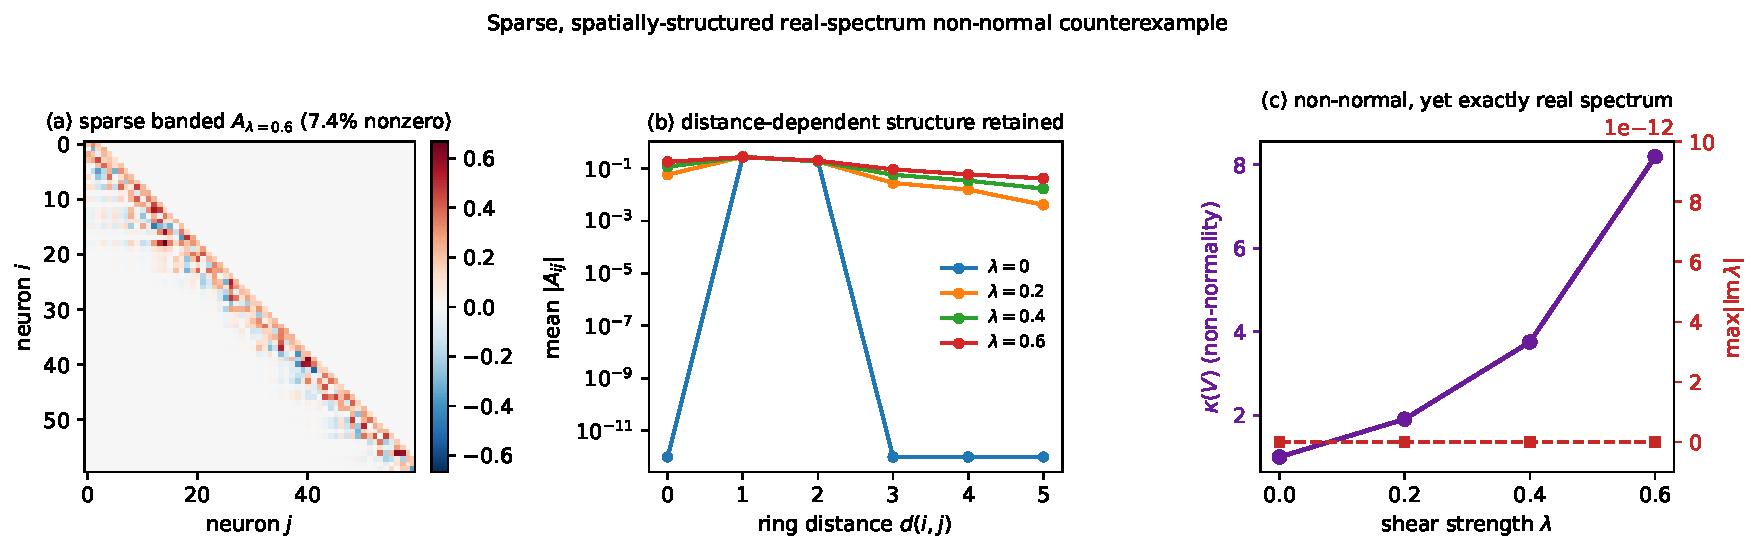
\includegraphics[width=\linewidth]{figures/ma_sparse_spatial.pdf}
\caption{\textbf{Exactly sparse, spatially structured real-spectrum non-normal
counterexample.} (a)~A representative diagonally transformed operator retains
the exact sparse support of its symmetric parent. (b)~Mean entry magnitude
retains a distance-dependent profile as gain heterogeneity increases.
(c)~Reciprocity falls and eigenvector non-normality grows without fill-in,
while the spectrum stays exactly real. Generated by
\texttt{ma\_sparse\_spatial\_\allowbreak counterexample.py}.}
\label{fig:supp-sparse}
\end{figure}

\section{Why functional recordings cannot resolve connectivity symmetry}
\label{sec:dataest}
One might hope to settle the question by estimating the effective operator $A$
directly from the recordings and reading off its non-normality. We provide a
turn-key pipeline for this
(\texttt{ma\_effective\_operator\_\allowbreak from\_data.py}: PCA
reduction, lag-one ridge regression $X_{t+1}\!\approx\!AX_t$, returning
$\kappa(V)$, $\eta$, $\max|\Im\lambda|$ and the abscissa gap
$\omega(A)-\alpha(A)$), and validate it on synthetic data with known ground truth
(Table~\ref{tab:dataest}). But this approach \emph{cannot} establish that cortical
connectivity is non-symmetric, for two independent reasons.

\emph{First, a level confound.} What is estimated from activity is the
\emph{effective} operator $A_{\mathrm{eff}}=GW_{\mathrm{syn}}$
(Sec.~\ref{sec:syn-eff}), not the synaptic matrix. Its non-normality does not
determine the symmetry of $W_{\mathrm{syn}}$: a symmetric $W_{\mathrm{syn}}$ with
heterogeneous gain yields a non-normal $A_{\mathrm{eff}}$, and conversely. A
measured $\kappa(V)\gg1$ would therefore no more prove asymmetric connectivity
than the Article's real DMD spectrum proves symmetric connectivity---it is the
same inference, reversed.

\emph{Second, an estimation floor.} The gap $\omega-\alpha$ (the
departure-from-normality gap: the largest eigenvalue of the operator's symmetric
part minus its spectral abscissa, which is nonnegative and whose positivity
certifies non-normality, although zero does not prove normality; computed here
on the estimated propagator rather than on a continuous-time generator)
separates the symmetric and non-normal validation families robustly
($\approx0$ versus $19$ in
Table~\ref{tab:dataest}), but $\kappa(V)$ estimated from finite data carries an
upward bias---a noise floor of $\kappa\!\approx\!30$ even for a \emph{truly
symmetric} operator---so it would have to be read against a symmetric-surrogate
null, and even then constrains only the effective operator. This floor is a
finite-sample effect, not fundamental: the validation in
Table~\ref{tab:dataest} uses only $N=120$, and the floor falls with neuron count
and recording length. Consequently the \emph{moderate} non-normality of the
$g{=}0.30$ counterexample (ideal $\kappa\approx6$, below the $N{=}120$ floor) is
not resolvable by $\kappa(V)$ at this small size but becomes resolvable in the
$N\sim10^3$--$10^4$ regime of cortical recordings; in this validation the gap
$\omega-\alpha$ is already robust at small $N$ and is the more reliable witness
when data are limited. The
proposed test thus flags \emph{sufficiently} non-normal effective operators,
with sensitivity to moderate non-normality improving as $N$ and $T$ grow.

These limits are not incidental; they are the identifiability boundary of the
main text, now in the other direction. The public recordings
(Figshare \texttt{janelia.27854448}) are \emph{entirely functional}---Neuropixels
spike trains and two-photon calcium fluorescence binned at $22$\,Hz, with no
structural-connectivity measurement. We therefore do \emph{not} analyze them to
argue for asymmetry: functional activity can no more establish that connectivity
is asymmetric than that it is symmetric. Resolving the question requires data the
recordings do not contain---direct structural connectivity (connectomics, paired
recordings) or causal perturbation responses that probe the recurrently dressed
susceptibility $\chi=(I-GW_{\mathrm{syn}})^{-1}G$ (Sec.~\ref{sec:syn-eff})---not a
re-analysis of the same functional observables.

\begin{table}[h]
\centering
\caption{Validation of the effective-operator estimator on synthetic data
($N=120$, matched real spectra). The estimator recovers the non-normality
witnesses from activity alone; $\omega-\alpha$ is the robust separator here.}
\label{tab:dataest}
\begin{tabular}{llccc}
\toprule
ground truth & source & $\kappa(V)$ & $\eta$ & $\omega-\alpha$\\
\midrule
\multirow{2}{*}{symmetric} & truth & $1.0$ & $1.000$ & $0.000$\\
 & from data & $29.6$ & $0.854$ & $0.008$\\
\multirow{2}{*}{non-normal (same spectrum)} & truth & $494$ & $-0.008$ & $29.7$\\
 & from data & $949$ & $0.004$ & $19.1$\\
\bottomrule
\end{tabular}
\end{table}

\section{Whole-connectome identifiability test on the FlyWire/Shiu model}
\label{sec:flywire}
The two gaps in the main text are arguments about what cannot be inferred from
functional observables. The FlyWire connectome supplies the one thing the mouse
recordings lack---structural connectivity, hence the reciprocity, as ground
truth---so it lets us test the inference directly in a nonlinear spiking network.
Three objects remain distinct throughout: the signed synaptic matrix $W$, the
nonlinear state-dependent LIF dynamics it drives, and the z-scored, partially
observed, PCA-reduced DMD propagator. They live in different coordinates and need
not share a reciprocity scalar; the test is whether the \emph{functional}
readouts move when the \emph{structural} reciprocity is varied with everything
else held fixed.

\subsection{Structural ground truth}
In the released graph ($N=127{,}400$; $14{,}687{,}178$ directed non-self edges),
density is $0.0905\%$ and $26.5\%$ of directed edges have a reverse edge---a
$293$-fold enrichment over independent support---yet the weighted reciprocity is
far from symmetric: $\eta_{\rm unsigned}=0.175$, $\eta_{\rm signed}=-0.041$, and
the topological reciprocated-edge fraction is $R=0.265$. The real connectome is
thus a strongly directed ground truth.

\subsection{Model and operating point}
We run the published Shiu LIF model\cite{shiu2024} with its recurrent parameters
fixed and add independent, balanced-E/I-like Poisson background streams to each
neuron. The excitatory/inhibitory event rates, their weight ratio and common
scale are calibrated only to place the model in a low, irregular spontaneous
regime; because a small high-rate tail strongly shifts the population mean,
operating points are screened jointly by median and upper-tail neuron rates,
silent fraction, per-neuron Fano factor and ten-block temporal stationarity,
never by a spectral outcome. The primary observable is binned spike count at
$\approx22$\,Hz; sampled membrane voltage is a secondary latent-state
diagnostic. We sweep a recurrence axis by a global multiplier $g$ on the
recurrent weights at fixed background, moving the network from
background-dominated ($g$ small; recurrence barely expressed) to
recurrence-dominated; lowering the background instead silences the network
(it sets the operating point), so the recurrence axis is climbed at fixed
background.

\subsection{Reciprocity controls at fixed degree}
The naive directionality control, direct symmetrization
$W_{\rm sym}=(W+W^\top)/2$ ($\eta=1$), is reported but is \emph{not} a clean
reciprocity manipulation: it nearly doubles the edge count
($2.5\times10^{7}$ edges, density $0.154\%$), so any functional difference
confounds reciprocity with density. We therefore add degree-preserving
Maslov--Sneppen nulls\cite{maslov2002}: directed target-swaps
$(a\!\to\!b),(c\!\to\!d)\mapsto(a\!\to\!d),(c\!\to\!b)$ that move only
postsynaptic targets, so each edge keeps its presynaptic neuron (hence its Dale
sign) and weight, and every neuron's in- and out-degree is preserved exactly.
Biasing acceptance toward or against reverse-edge creation tunes reciprocity
while holding degree, weight multiset and Dale sign fixed. This yields two
density-matched nulls, \texttt{degree\_randomized} ($R=0.006$) and
\texttt{degree\_reciprocal} ($R=0.690$), that bracket the real value
($R=0.265$); a perfectly symmetric $\eta=1$ graph is \emph{impossible} at fixed
degree (it forces $\mathrm{in}_i=\mathrm{out}_i$), which is exactly why
$W_{\rm sym}$ must change density. We verified that both nulls preserve the in-
and out-degree sequences and the signed-weight multiset exactly. The null graph
is built once (fixed graph seed) and reused across simulation seeds, so error
bars reflect background noise, matching the other controls.

\subsection{Functional analysis}
The functional analysis directly calls the pinned public
\texttt{MouseLand/critical\_init} implementations of random-split
\texttt{SVCA2}, \texttt{fit\_powerlaw\_exp}, and PCA-reduced \texttt{lyapun.dmd}
at a $0.23$\,s lag (commit verified at load time). We report the exponent $\nu$,
rotations per tenfold attenuation, the maximum imaginary eigenvalue part
$\max|\Im\lambda|$, and the eigenvector condition number. These are descriptors
of the fitted propagator, not estimates of synaptic reciprocity.

\subsection{Result: neither observable recovers reciprocity}
At the background-dominated operating point all controls are indistinguishable
on every readout (including, after rate-matched neuron subsampling, the exponent:
$\Delta\nu=-0.011\pm0.004$ between original and symmetrized), so any sensitivity
must emerge under strong recurrence. It does not, in the way the original
inference requires (Table~\ref{tab:flywire}):

\emph{(i) The DMD spectral readout is blind to reciprocity.} Across the
density-matched controls---reciprocity from $R=0.006$ to $0.69$, bracketing the
real $0.265$---the imaginary content is flat, $\max|\Im\lambda|\approx0.167$, and
modal rotation is $\approx0$, regardless of reciprocity. This is the empirical
form of Gap~2 in a spiking network with ground truth. Rotation appears only when
the \emph{symmetric} null is driven into a synchronous regime, where the
perfectly symmetric ($\eta=1$) graph reliably yields a strongly rotating
functional spectrum across all three seeds ($\max|\Im\lambda|\approx0.5$,
rotation $1.4$--$2.0$)---the converse failure
running the opposite way (symmetric structure $\to$ complex functional spectrum),
complementing the analytic counterexample of Sec.~\ref{sec:counterexample}
(asymmetric structure $\to$ real spectrum).

\emph{(ii) The exponent does not track reciprocity.} For all three
density-matched graphs $\nu$ rises with recurrence over $8$--$18$\,Hz
($\nu\approx0.2$--$0.5$); only the density-doubled symmetrized null is pinned
flat at $\nu\approx0.13$ and does not respond to recurrence at all. Its apparent
$\nu$ ``separation'' from the real network is therefore a density effect, not a
reciprocity effect. Among the density-matched controls the exponent does not
isolate reciprocity: at matched rate the real network ($R=0.265$) and the
high-reciprocity null ($R=0.69$) coincide ($\nu=0.24$ vs $0.21$ at
$\sim$10\,Hz), and at $18$\,Hz the real network ($\nu=0.46$) \emph{exceeds} the
most reciprocal null ($\nu=0.36$), so $\nu$ reflects operating point and gross
topology, not $R$. This is the empirical form of Gap~1. Moreover, reciprocity
and operating point cannot be set independently---raising reciprocity raises the
gain-to-rate efficiency, so matching firing rate forces a different effective
coupling---which is precisely the $\nu(\eta,\alphaeff)$ degeneracy of
Sec.~\ref{sec:degeneracy} made concrete.

\begin{table}[h]
\centering
\caption{Functional readouts versus structural reciprocity in the FlyWire/Shiu
model. The three density-matched controls span reciprocity over two orders of
magnitude at fixed in/out-degree, weight multiset and Dale sign; the symmetrized
null is $\eta=1$ but doubles density. $\max|\Im\lambda|$ is flat across the
reciprocity range; $\nu$ rises with recurrence for every density-matched graph
and is pinned only for the density-doubled null.}
\label{tab:flywire}
\begin{tabular}{lccccc}
\toprule
control & $R$ & density & $\max|\Im\lambda|$ & rotation & $\nu$ (binned)\\
\midrule
degree-null (recip.\ $\downarrow$) & $0.006$ & $0.091\%$ & $0.169$ & $0$ & $0.21$--$0.45^{\ddagger}$\\
original (real) & $0.265$ & $0.091\%$ & $0.168$ & $0$ & $0.24$--$0.47^{\ddagger}$\\
degree-null (recip.\ $\uparrow$) & $0.690$ & $0.091\%$ & $0.167$ & $0$ & $0.21$--$0.36^{\ddagger}$\\
symmetrized & $1.000$ & $0.154\%$ & $0.172\,(\sim0.5^{\dagger})$ & $0\,(1.4\text{--}2.0^{\dagger})$ & $\approx0.13$ (flat)\\
\bottomrule
\end{tabular}

\smallskip
{\footnotesize $^{\ddagger}$ rises with recurrence over the $8$--$18$\,Hz range.
\quad $^{\dagger}$ synchronous high-gain regime.}
\end{table}

\subsection{Scope}
This is a proof of principle with structural ground truth in \emph{Drosophila},
not a claim about mouse cortex: it shows that the Article's functional readouts
fail to recover known connectivity reciprocity in a biophysical spiking network,
exactly as the two gaps predict. As in Sec.~\ref{sec:dataest}, the readouts
constrain a partially observed, gain-dressed effective propagator, not the
synaptic matrix; the controls here additionally hold density and degree fixed, so
the failure cannot be dismissed as an operating-point or scale artifact. The
implementation, controls and server workflow are in
\texttt{flywire\_spontaneous/}.

\section{Reproducibility}
All results and the main figure are reproduced by:
\begin{verbatim}
python ma_degeneracy_surface.py
python ma_real_spectrum_counterexample.py
python ma_sparse_spatial_counterexample.py
python ma_effective_operator_from_data.py
python make_fig_v4.py
cd ../flywire_spontaneous
bash setup_critical_init.sh
bash download_data.sh
# build the degree-preserving reciprocity nulls (cached)
python connectome_controls.py --con 2023_03_23_connectivity_630_final.parquet \
       --control degree_reciprocal
python connectome_controls.py --con 2023_03_23_connectivity_630_final.parquet \
       --control degree_randomized
# recurrence ladder + per-control SVCA2/DMD scans (across GPUs), then the figure
GPU_IDS="0 6 7" bash sweep_recurrence.sh
CONTROL=degree_reciprocal GAINS="1.5 2.0 2.5" bash iso_nu_search.sh
CONTROL=degree_randomized GAINS="1.5 2.0 2.5" bash iso_nu_search.sh
python make_fig_identifiability.py iso_*_analysis.json spont_poisson_recdom*_analysis.json \
       --R original=0.265 symmetrized=1.0 degree_reciprocal=0.690 degree_randomized=0.006 \
       --out ../nature_matters_arising/figures/fig_identifiability
\end{verbatim}
The numerical outputs are stored in \texttt{ma\_degeneracy\_surface.json} and
\texttt{ma\_real\_spectrum\_results.json}, with validation data in
\texttt{ma\_probe\_diagnostic.py} and \texttt{ma\_controls.py}. The sparse,
spatially-structured counterexample (Sec.~\ref{sec:sparse}) and the turn-key
effective-operator estimator and its synthetic validation (Sec.~\ref{sec:dataest})
are reproduced by the third and fourth scripts.

\begin{thebibliography}{99}
\bibitem{pachitariu2026}
M.~Pachitariu, L.~Zhong, A.~Gracias, A.~Minisi, C.~Lopez, C.~Stringer,
``A critical initialization for biological neural networks,''
\emph{Nature} (2026).

\bibitem{shiu2024}
P.~K.~Shiu et al.,
``A Drosophila computational brain model reveals sensorimotor processing,''
\emph{Nature} \textbf{634}, 210--219 (2024).

\bibitem{maslov2002}
S.~Maslov, K.~Sneppen,
``Specificity and stability in topology of protein networks,''
\emph{Science} \textbf{296}, 910--913 (2002).

\bibitem{sommers1988}
H.~J.~Sommers, A.~Crisanti, H.~Sompolinsky, Y.~Stein,
``Spectrum of large random asymmetric matrices,''
\emph{Phys.\ Rev.\ Lett.} \textbf{60}, 1895--1898 (1988).

\bibitem{trefethen2005}
L.~N.~Trefethen, M.~Embree,
\emph{Spectra and Pseudospectra},
Princeton University Press (2005).

\bibitem{hornjohnson2013}
R.~A.~Horn, C.~R.~Johnson,
\emph{Matrix Analysis}, 2nd ed.,
Cambridge University Press (2013).

\bibitem{wigner1958}
E.~P.~Wigner,
``On the distribution of the roots of certain symmetric matrices,''
\emph{Ann.\ Math.} \textbf{67}, 325--327 (1958).

\bibitem{sompolinsky1988}
H.~Sompolinsky, A.~Crisanti, H.~J.~Sommers,
``Chaos in random neural networks,''
\emph{Phys.\ Rev.\ Lett.} \textbf{61}, 259--262 (1988).

\bibitem{rajan2006}
K.~Rajan, L.~F.~Abbott,
``Eigenvalue spectra of random matrices for neural networks,''
\emph{Phys.\ Rev.\ Lett.} \textbf{97}, 188104 (2006).

\bibitem{schmid2010}
P.~J.~Schmid,
``Dynamic mode decomposition of numerical and experimental data,''
\emph{J.\ Fluid Mech.} \textbf{656}, 5--28 (2010).

\bibitem{murphy2009}
B.~K.~Murphy, K.~D.~Miller,
``Balanced amplification,''
\emph{Neuron} \textbf{61}, 635--648 (2009).

\bibitem{goldman2009}
M.~S.~Goldman,
``Memory without feedback in a neural network,''
\emph{Neuron} \textbf{61}, 621--634 (2009).

\bibitem{hennequin2014}
G.~Hennequin, T.~P.~Vogels, W.~Gerstner,
``Optimal control of transient dynamics in balanced networks,''
\emph{Neuron} \textbf{82}, 1394--1406 (2014).

\bibitem{bondanelli2020}
G.~Bondanelli, S.~Ostojic,
``Coding with transient trajectories in recurrent neural networks,''
\emph{PLoS Comput.\ Biol.} \textbf{16}, e1007655 (2020).

\bibitem{chau2025}
H.~Y.~Chau, K.~D.~Miller, A.~Palmigiano,
``Exact linear theory of perturbation response in a space- and feature-dependent
cortical circuit model,''
\emph{Proc.\ Natl.\ Acad.\ Sci.\ U.S.A.} \textbf{122}, e2426758122 (2025).
\end{thebibliography}

\end{document}
